\interlude{Endzeitstimmung}

\begin{frame}[T]{Die Zerstörung der Kryptografie}
% "Warum sind wir eigentlich hier"
% Todo (Karo): Reisserische Youtube Headings Einfügen
%\begin{itemize}
  % \item \url{https://www.youtube.com/watch?v=e-lIgqD5Nxk}
  % \item \url{https://www.youtube.com/watch?v=h6w4SX7ZJMQ}
  % \item \url{https://www.youtube.com/watch?v=-UrdExQW0cs}
  % \item \url{https://www.youtube.com/watch?v=05Uy-hFFkRU}
  % \item \url{https://www.youtube.com/watch?v=ON5pVc9bIRo}
    % - "Lehrer: Subjekt, prädikat, objekt – Der Satz ist unvollständig"
  % - Hier geht es viel um Bitcoiin.
    % - Wir kryptografen sind ja nicht so glücklich darüber, dass die Bitcoin-Bros uns das Kürzel gestohlen haben
% \end{itemize}
\only<1>{
  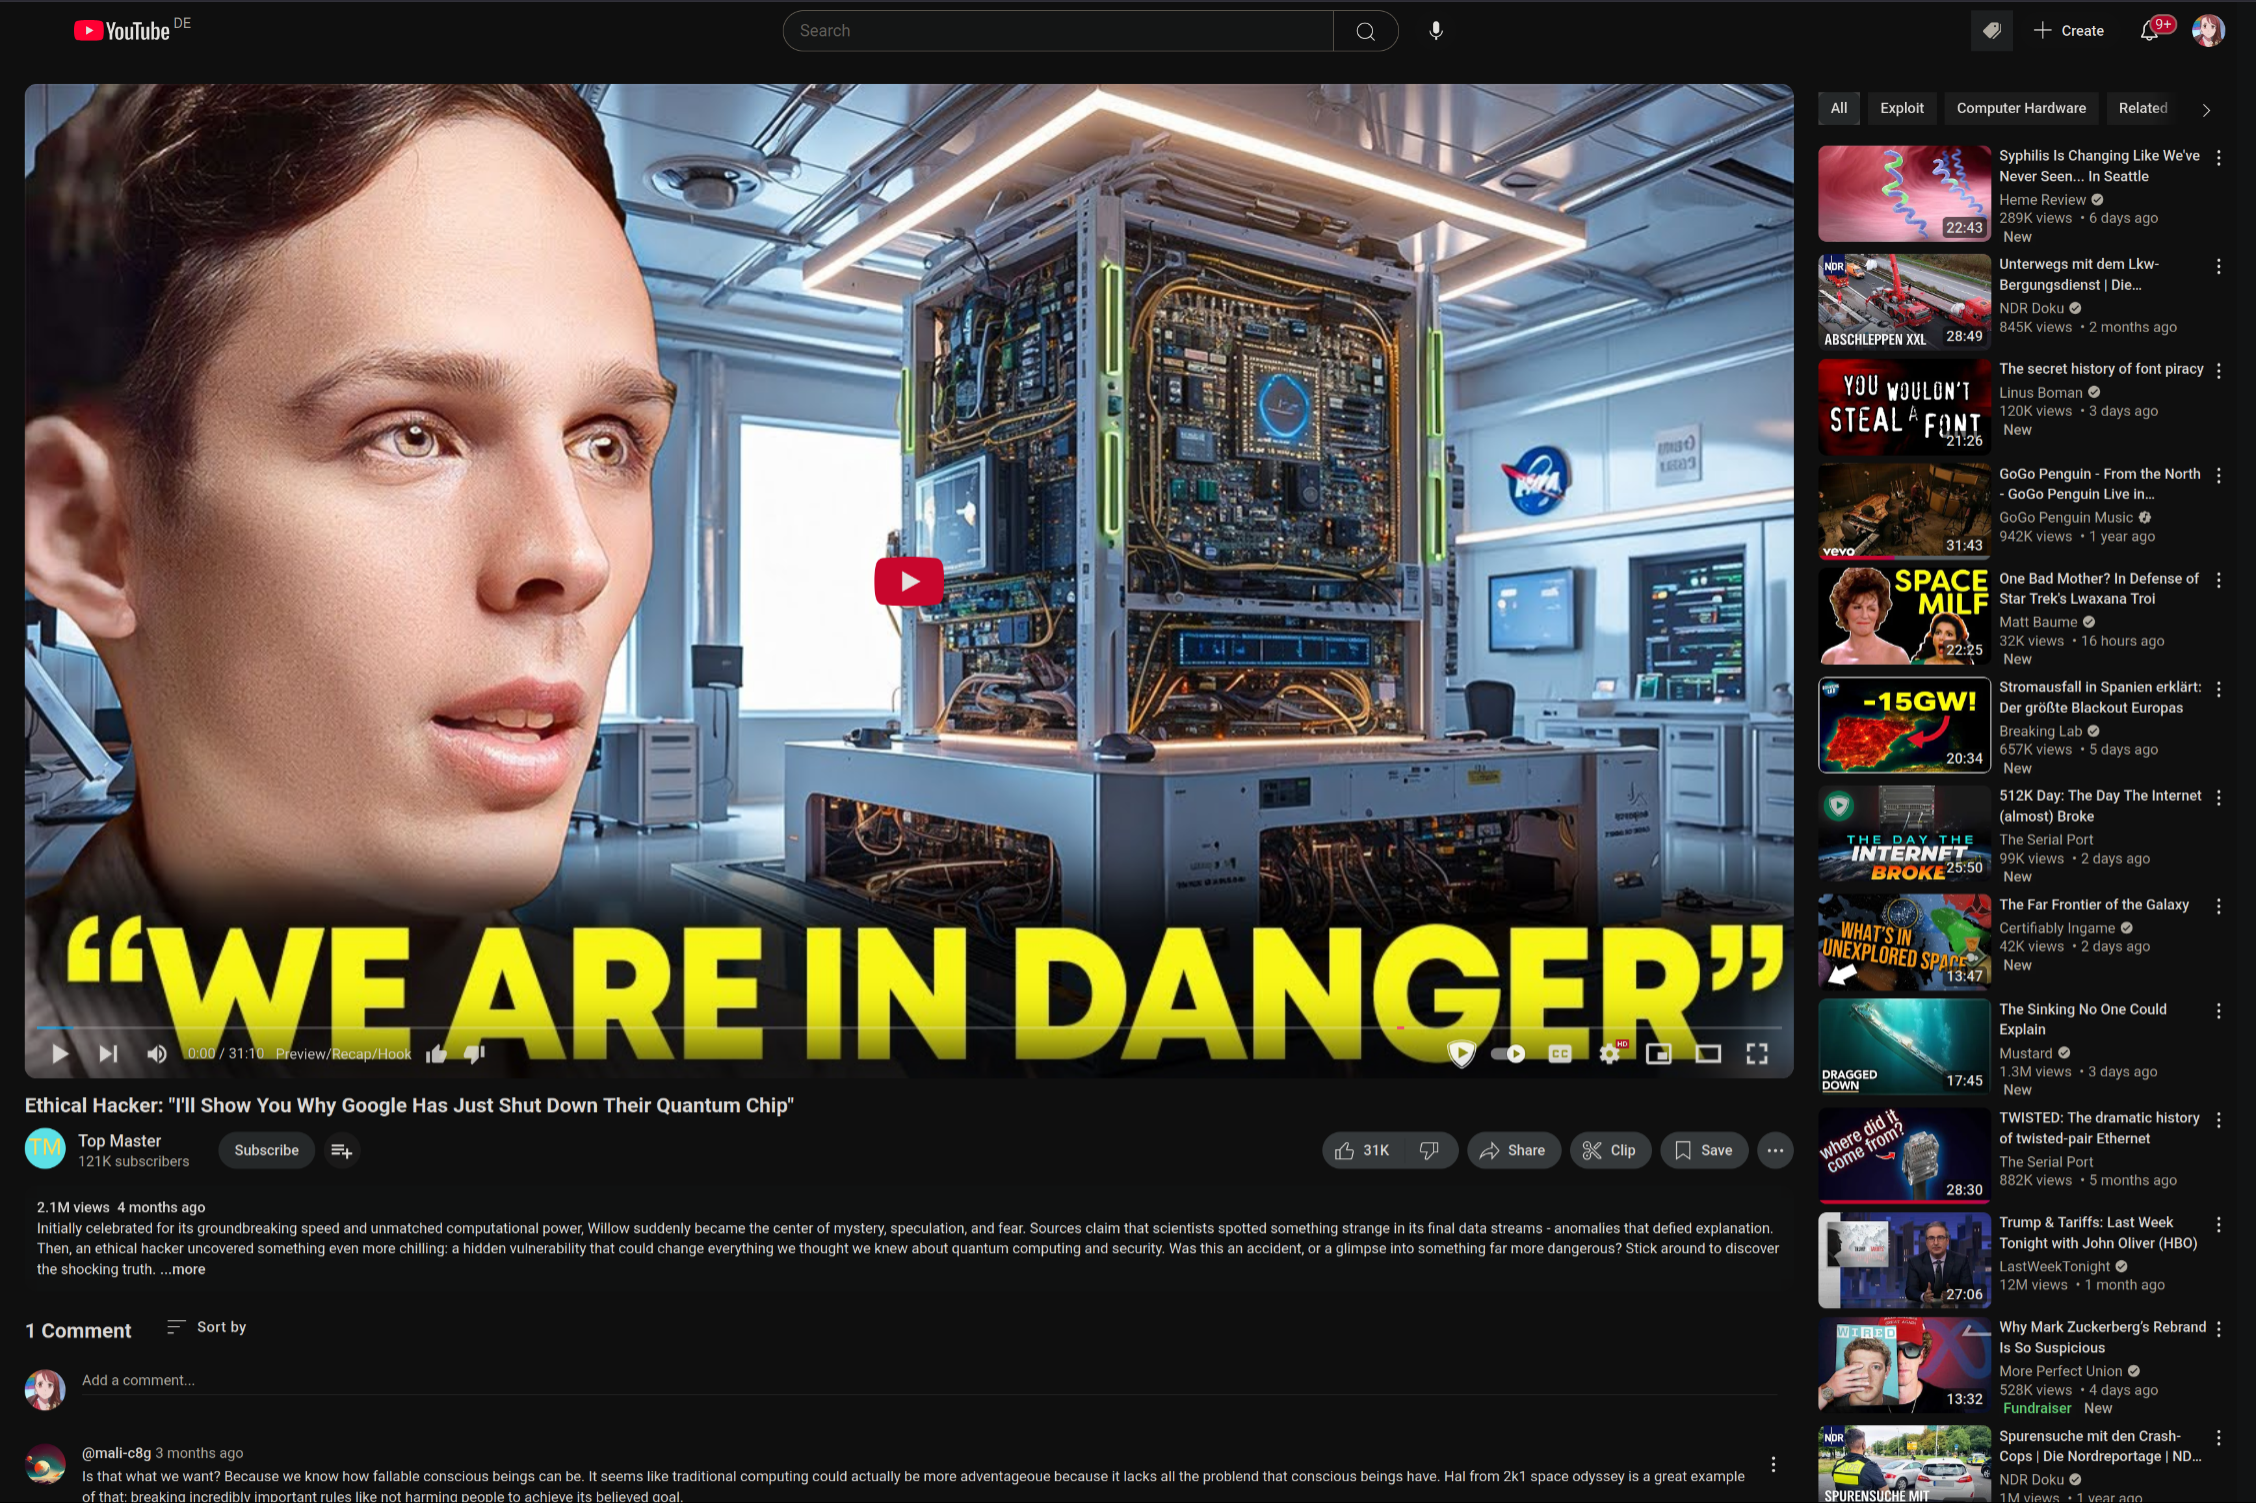
\includegraphics[width=.98\linewidth,trim=10 350 400 62,clip]{graphics/quantastropy-yt-screenshots/we-are-in-danger.png}
  Quelle: \url{https://www.youtube.com/watch?v=h6w4SX7ZJMQ}
}
\only<2>{
  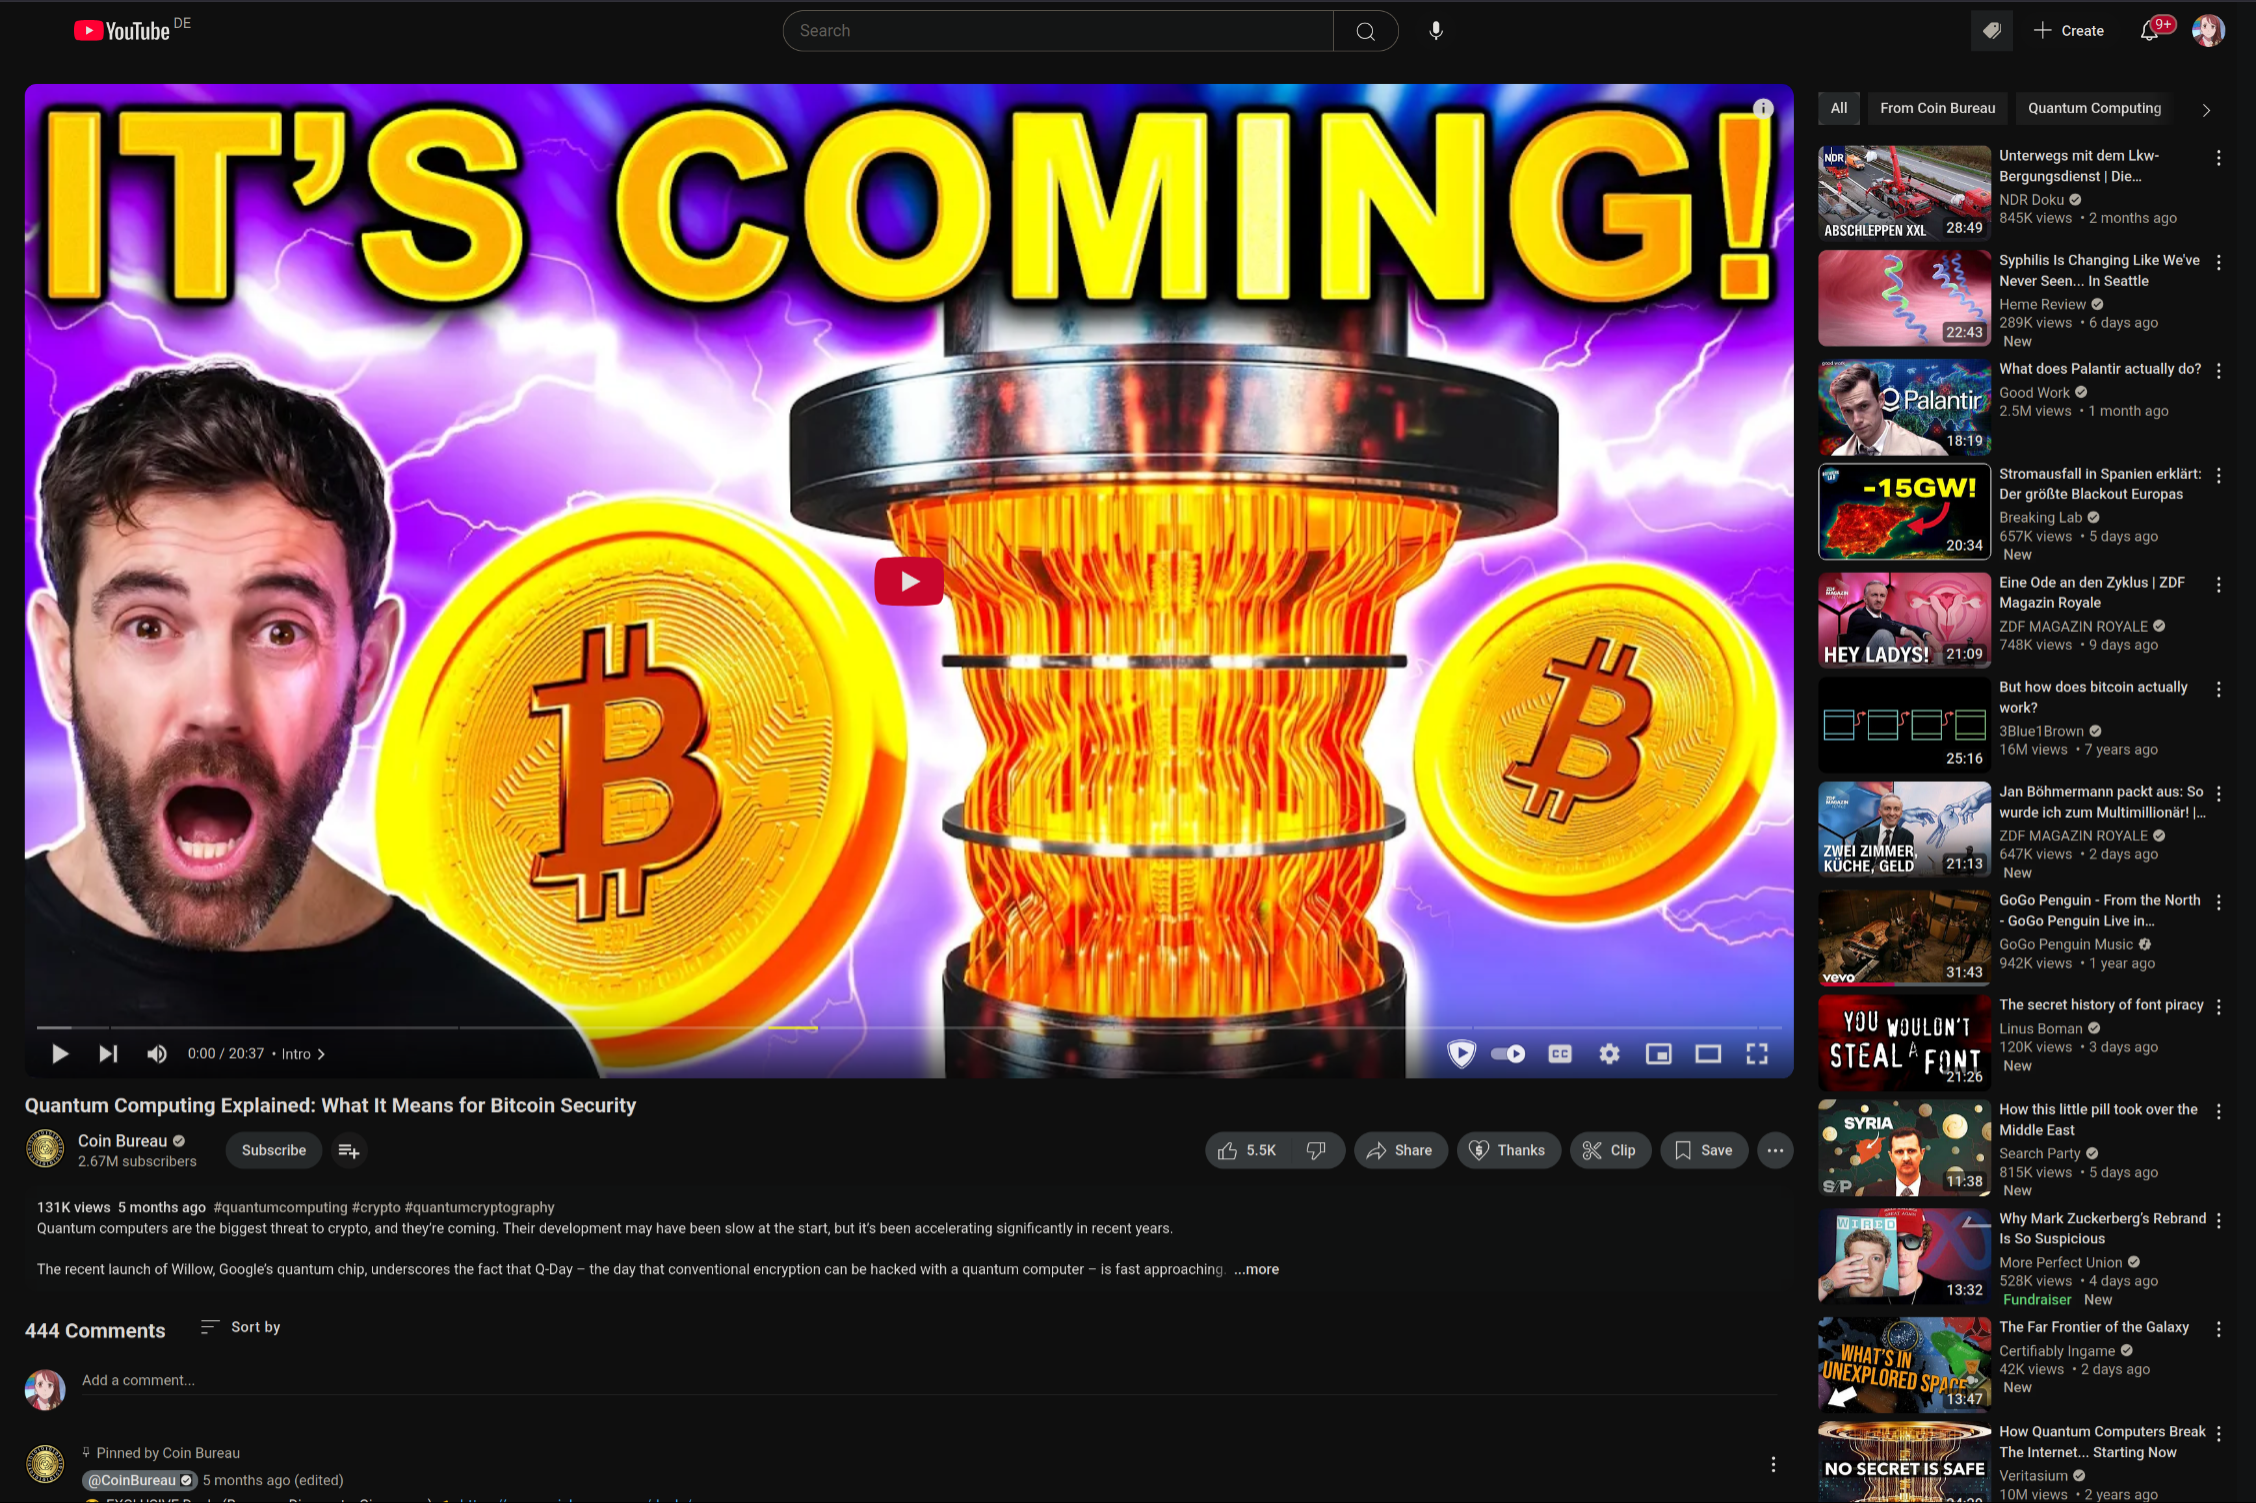
\includegraphics[width=.98\linewidth,trim=10 350 400 62,clip]{graphics/quantastropy-yt-screenshots/it-is-coming.png}
  Quelle: \url{https://www.youtube.com/watch?v=ON5pVc9bIRo}
}
\only<3>{
  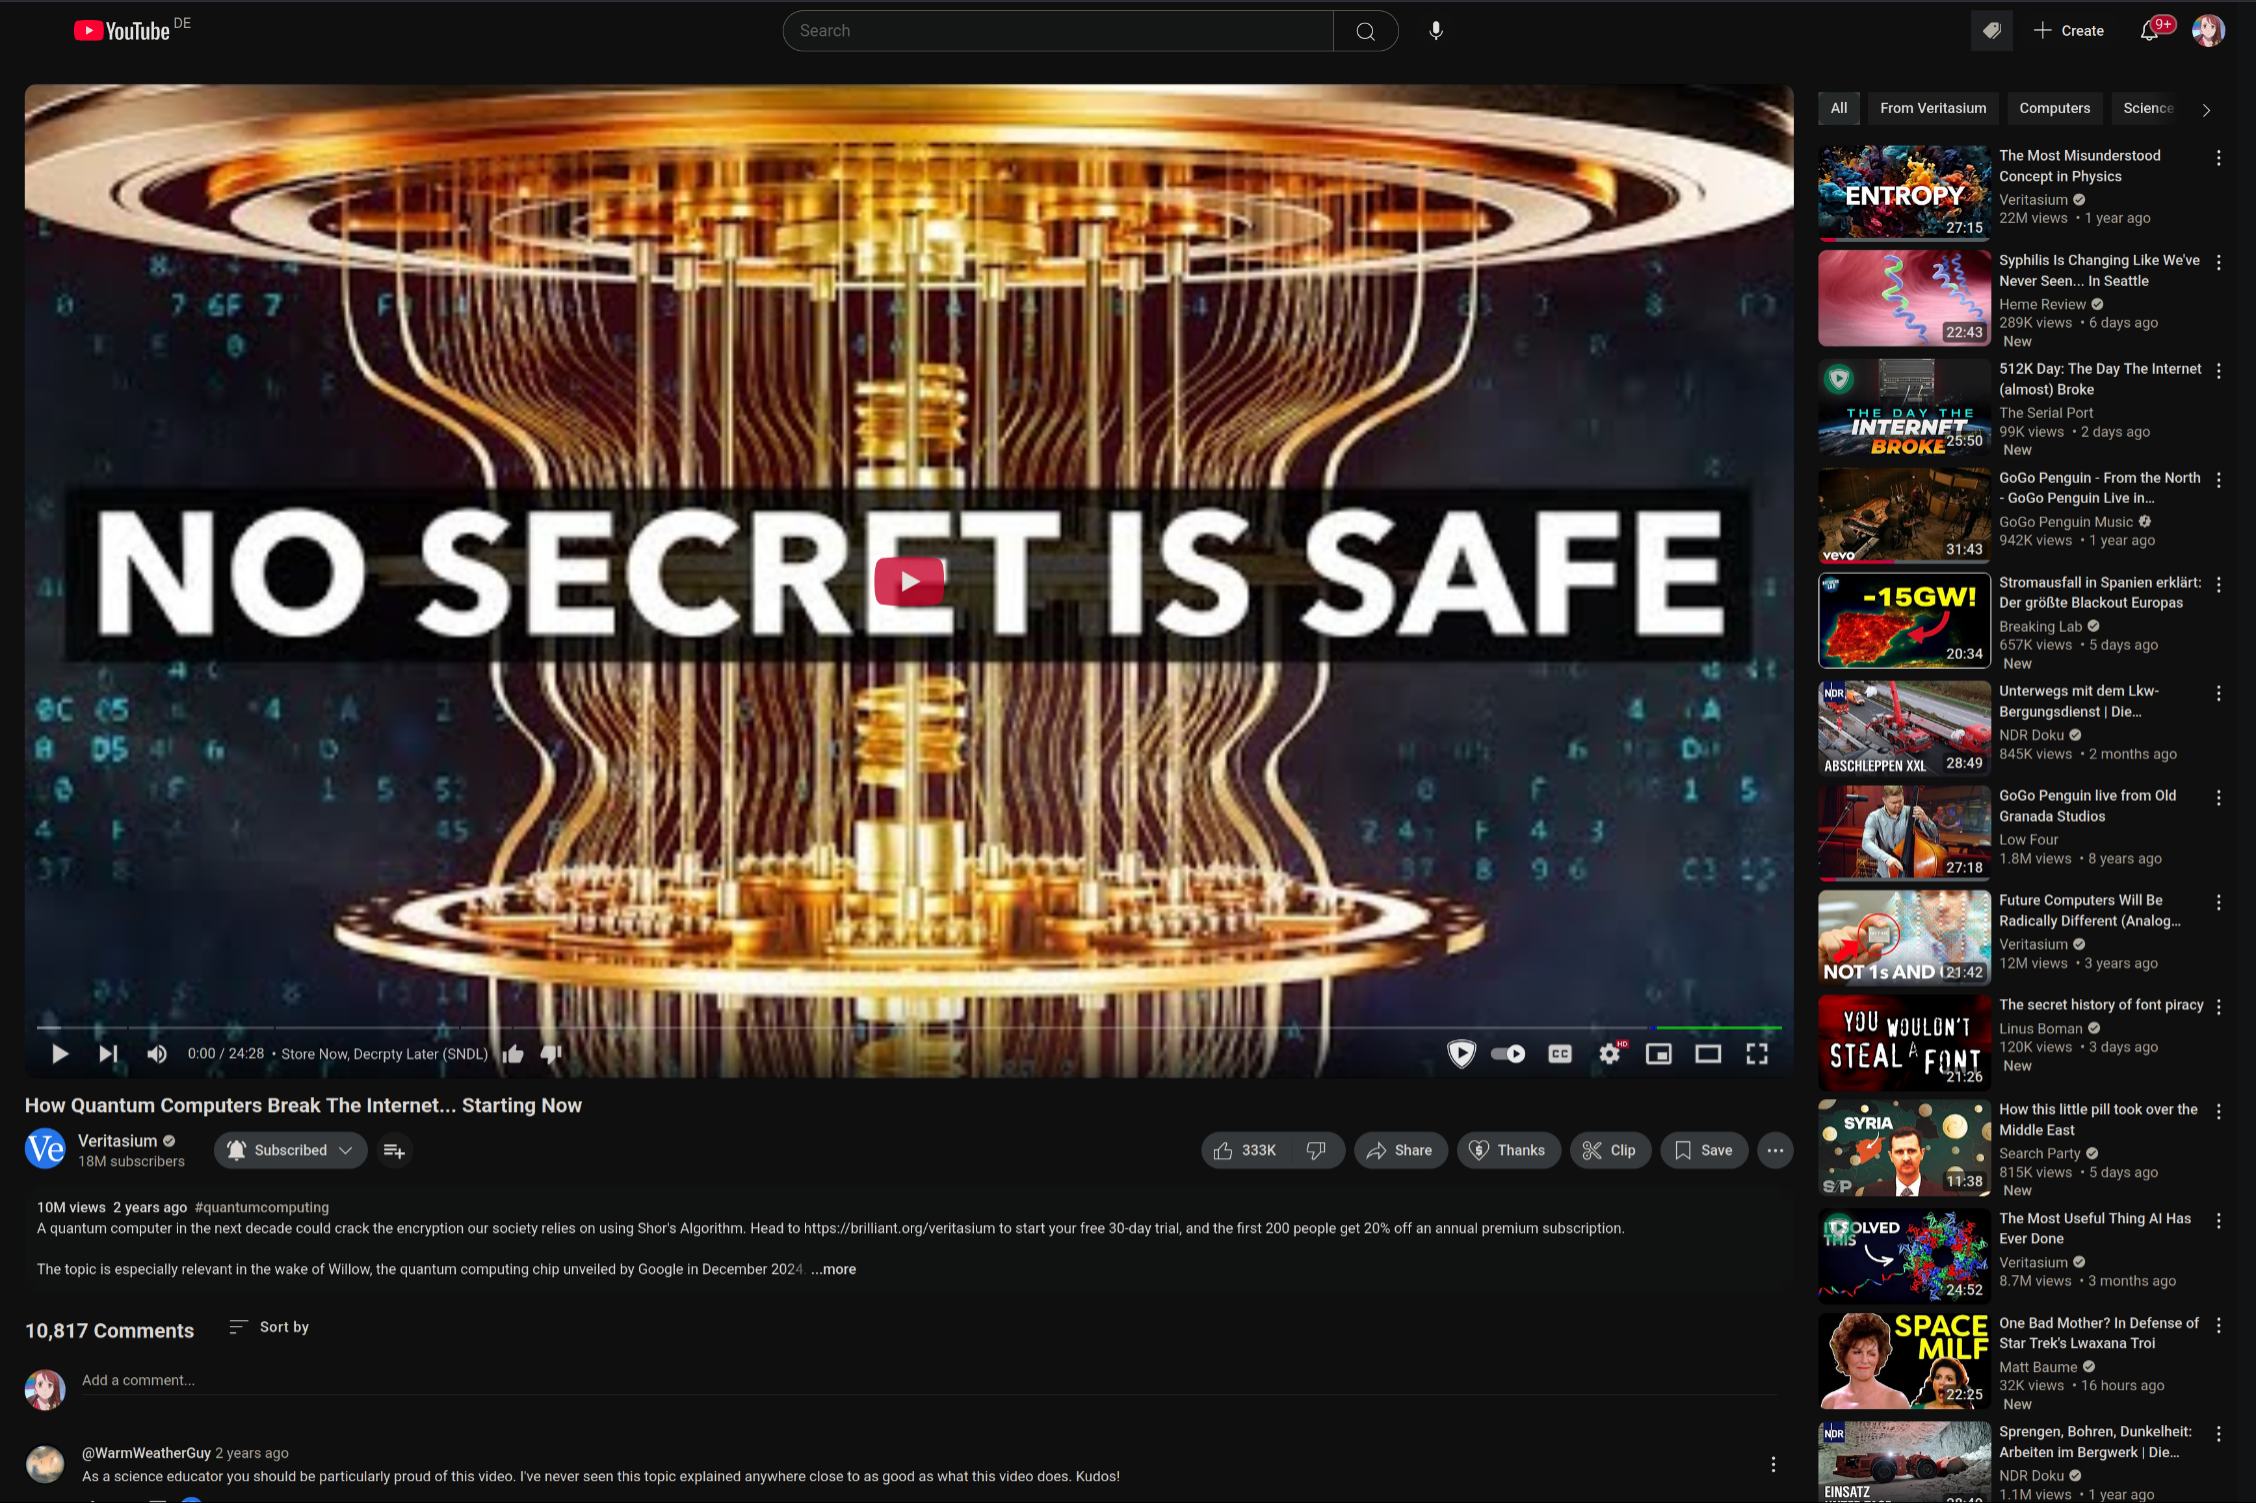
\includegraphics[width=.98\linewidth,trim=10 350 400 62,clip]{graphics/quantastropy-yt-screenshots/no-secret-is-safe.png}
  Quelle: \url{https://www.youtube.com/watch?v=-UrdExQW0cs}
}
\end{frame}

% \begin{frame}[T]{Quantencomputer – Shors Algorithmus}

% \begin{itemize}
%   \item Kann speziefische Kryptografische Primitiven Angreifen
%   \item Schneller als Exponenziell
%   \item Erfunden 1994
%   \item Gegenmaßnahme existieren seit 1978 (das wussten wir damals nur nicht)
%   \item Es ist teuer und komplex die in den Einsatz zu bringen
%   \item => Diese komponenten werden Flächendeckend eingesetzt
% \end{itemize}

% Bild: 
% \begin{itemize}
%   \item Physiker: Mein Gerät lässt Flugzeuge mit RS 25 McGuffin Triebwerken abstürzen
%   \item Manager: RS 26 McGuffin Triebwerke sind so viel teurer. Niemand wird migrieren wollen.
%   \item Physiker: Halt dich ran, ich brauche nur 40 Jahre um das zu bauen!
% \end{itemize}

% \end{frame}

\begin{frame}[T]{Quantencomputer – So schnell wie Fusion}
  
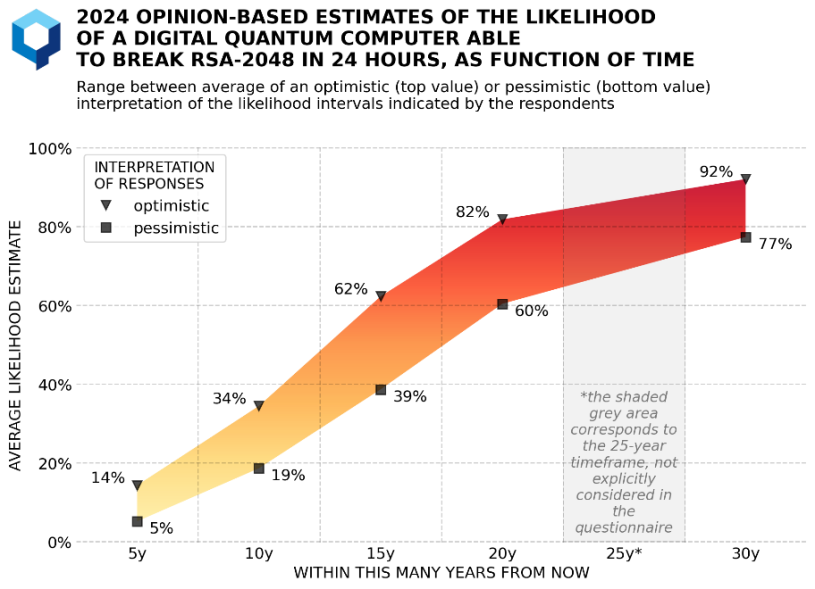
\includegraphics[width=.92\linewidth,clip,trim=0  0 0 120]{graphics/quantum-timeline.png}
Quelle: \url{https://globalriskinstitute.org/publication/2024-quantum-threat-timeline-report/}

\end{frame}


\begin{frame}[T]{Quantencomputer – Ein Risiko Besteht}

Bild: Erde Stoppt
\begin{itemize}
  \item "Ahh wir haben vergessen die Erde zu tanken"
  \item "Hmm, riecht nach huhn" (helle seite)
  \item "Yeah, schlitten fahren" (dunkle seite)
  \item "Technoparty, die ewige nacht lang" (dunkle seite)
\end{itemize}

\end{frame}


\begin{frame}[T]{Quantencomputer – Jetzt speichern, später angreifen}

Bild: Store now decrypt later attack

\end{frame}
